\documentclass[11pt]{article}
\usepackage[width=7.5in, height=9.5in, top=0.5in, papersize={8.5in,11in}]{geometry}
\usepackage{ulem}
\usepackage[dvipsnames,svgnames]{xcolor}
\usepackage[pdftex]{graphicx}
\usepackage{pdfpages}
\title{SDSMT SENIOR DESIGN SOFTWARE DEVELOPMENT AGREEMENT}
\usepackage{hyperref}
\setlength{\parskip}{2mm}
\setlength{\parindent}{0mm}


\begin{document}
\typeout{"This is the Software Agreement.  Take this seriously!"}


{\Large \bf 
\centerline{SDSMT SENIOR DESIGN}\centerline{SOFTWARE DEVELOPMENT AGREEMENT}
}
\vspace{\baselineskip}

This Software Development Agreement (the ``Agreement") is made between the SDSMT  Computer Science Senior Design Team ``Crowd Science Mapper'',
consisting of team members Hannah Aker and Jiasong Yan, 
 and  Sponsors  Dr.Mengyu Qiao and Gail Schmidt, 
 with address: 501 E. Saint Joeseph Street, Rapid City, SD, 57701. 

\section{RECITALS}
\begin{enumerate}  \itemsep4pt \parskip0pt \parsep0pt
\item Sponsor desires Senior Design Team to develop a set of generic crowdsourcing system framework and toolkits, which can be customized by ordinary users with no programming experience using graphical user interface.    

\item Senior Design Teams willing to develop such Software.  
\end{enumerate}
NOW, THEREFORE, in consideration of the mutual covenants and promises herein contained, the Team and Sponsor agree as follows:  

\section{EFFECTIVE DATE }

This Agreement shall be effective as of September 14, 2015.  

\section{DEFINITIONS }
\begin{enumerate}  \itemsep4pt \parskip0pt \parsep0pt
\item ``Software" shall mean the computer programs in machine readable object code form and any subsequent error corrections or updates supplied to Sponsor by Senior Design Team pursuant to this Agreement.

\end{enumerate}

\section{DEVELOPMENT OF SOFTWARE }
\begin{enumerate}  \itemsep4pt \parskip0pt \parsep0pt
\item  Senior Design Team will use its best efforts to develop the Software described in the Crowd Science Mapper project description. The Software development will be under the direction of  or his/her successors as mutually agreed to by the parties (``Team Lead") and will be conducted by the Team Lead.  The Team will deliver the Software to the satisfaction of the course instructor that reasonable effort has been made to address the needs of the client.  The Team understands that failure to deliver the Software is grounds for failing the course. 

\item  Sponsor understands that the Senior Design course's mission is education and advancement of knowledge, and, consequently, the development of Software must further that mission. The Senior Design Course does not guarantee specific results or any results, and the Software will be developed only on a best efforts basis.  The Software is considered PROOF OF CONCEPT only and is NOT intended for commercial, medical, mission critical or industrial applications.

\item  The Senior Design instructor will act as mediator between Sponsor and Team; and resolve any conflicts that may arise.
\end{enumerate}

\section{COMPENSATION}

No Compensation

\section{CONSULTATION AND REPORTS}     
\begin{enumerate}  \itemsep4pt \parskip0pt \parsep0pt
\item  Sponsor's designated representative for consultation and       communications with the Team Lead shall be Dr. Mengyu Qiao    or such other person as Sponsor       may from time to time designate to the Team Lead (``Designated Representative").    

\item During the Term of the Agreement, Sponsor's representatives may       consult informally with course instructor regarding the       project, both personally and by telephone. Access to work carried       on in University facilities, if any, in the course of this Agreement shall       be entirely under the control of University personnel but shall be       made available on a reasonable basis.    

\item The Team Lead will submit written progress reports. At the conclusion of this Agreement, the Team Lead shall submit a comprehensive final report in the form of the formal course documentation at the conclusion of the Senior Design II course. 
\end{enumerate}

\section{CONFIDENTIAL INFORMATION }    
\begin{enumerate}  \itemsep4pt \parskip0pt \parsep0pt
\item The parties may wish, from time to time, in connection with work       contemplated under this Agreement, to disclose confidential       information to each other (``Confidential Information"). Each party       will use reasonable efforts to prevent the disclosure of any of       the other party's Confidential Information to third parties for a       period of three (3) years after the termination of this Agreement,       provided that the recipient party's obligation shall not apply to       information that:               
\begin{enumerate}  \itemsep4pt \parskip0pt \parsep0pt
\item  is not disclosed in writing or reduced to writing and so                 marked with an appropriate confidentiality legend within                 thirty (30) days of disclosure;              
\item is already in the recipient party's possession at the                 time of disclosure thereof;              
\item  is or later becomes part of the public domain through no                 fault of the recipient party;              
\item  is received from a third party having no obligations of                 confidentiality to the disclosing party;              
\item is independently developed by the recipient party; or              
\item is required by law or regulation to be disclosed.     
\end{enumerate}
\item In the event that information is required to be disclosed pursuant       to subsection (6), the party required to make disclosure shall       notify the other to allow that party to assert whatever exclusions       or exemptions may be available to it under such law or regulation.  
\end{enumerate}


\section{INTELLECTUAL PROPERTY RIGHTS } 

All deliverables become property of South Dakota School of Mines and Technology.

\section{WARRANTIES }  

The Senior Design Team represents and warrants to Sponsor that:         
\begin{enumerate}  \itemsep4pt \parskip0pt \parsep0pt
\item  the Software is the original work of the Senior Design Team in each and all aspects;        

\item the Software and its use do not infringe any copyright or   trade secret rights of any third party.  
\end{enumerate}
No agreements will be made beyond items (1) and (2).

\section{INDEMNITY}   
\begin{enumerate}  \itemsep4pt \parskip0pt \parsep0pt
\item Sponsor is responsible for claims and damages, losses or expenses held against the Sponsor. 

\item  Sponsor shall       indemnify and hold harmless the Senior Design Team, its affiliated companies       and the officers, agents, directors and employees of the same from       any and all claims and damages, losses or expenses, including       attorney's fees, caused by any negligent act of Sponsor or any of       Sponsor's agents, employees, subcontractors, or suppliers.    

\item  NEITHER PARTY TO THIS AGREEMENT NOR THEIR AFFILIATED COMPANIES,       NOR THE OFFICERS, AGENTS, STUDENTS AND EMPLOYEES OF ANY OF THE       FOREGOING, SHALL BE LIABLE TO ANY OTHER PARTY HERETO IN ANY ACTION       OR CLAIM FOR CONSEQUENTIAL OR SPECIAL DAMAGES, LOSS OF PROFITS,       LOSS OF OPPORTUNITY, LOSS OF PRODUCT OR LOSS OF USE, WHETHER THE       ACTION IN WHICH RECOVERY OF DAMAGES IS SOUGHT IS BASED ON CONTRACT       TORT (INCLUDING SOLE, CONCURRENT OR OTHER NEGLIGENCE AND STRICT       LIABILITY), STATUTE OR OTHERWISE. TO THE EXTENT PERMITTED BY LAW,       ANY STATUTORY REMEDIES WHICH ARE INCONSISTENT WITH THE PROVISIONS       OF THESE TERMS ARE WAIVED.  
\end{enumerate}

\section{INDEPENDENT CONTRACTOR}  

For the purposes of this Agreement and all services to be provided hereunder, the parties shall be, and shall be deemed to be, independent contractors and not agents or employees of the other party. Neither party shall have authority to make any statements, representations or commitments of any kind, or to take any action which shall be binding on the other party, except as may be expressly provided for herein or authorized in writing.  

\section{TERM AND TERMINATION }    
\begin{enumerate}  \itemsep4pt \parskip0pt \parsep0pt
\item This Agreement shall commence on the Effective Date and extend until the end of classes of the second semester of Senior Design (CSC 465), unless sooner terminated in accordance with the provisions of this Section (``Term"). 

\item This Agreement may be terminated by the written agreement of both       parties.    

\item In the event that either party shall be in default of its       materials obligations under this Agreement and shall fail to       remedy such default within thirty (30) days after receipt of       written notice thereof, this Agreement shall terminate upon       expiration of the thirty (30) day period.    

\item Any provisions of this Agreement which by their nature extend       beyond termination shall survive such termination.  
\end{enumerate}


\section{ATTACHMENTS}  

Attachment ``Crowd Science Mapper Project Description'' is incorporated in this Agreement.  

\section{GENERAL }    
\begin{enumerate}  \itemsep4pt \parskip0pt \parsep0pt
\item This Agreement constitutes the entire and only agreement between       the parties relating to the Senior Design Course, and all prior       negotiations, representations, agreements and understandings are       superseded hereby. No agreements altering or supplementing the       terms hereof may be made except by means of a written document       signed by the duly authorized representatives of the parties.    

\item This Agreement shall be governed by, construed, and enforced in       accordance with the internal laws of the State of South Dakota. 
\end{enumerate}

\section{SIGNATURES}    
\begin{tabular}{ll}
  \strut\vspace{0.25in} & \\
  \makebox[3in]{\hrulefill} & \makebox[2in]{\hrulefill} \\
  Hannah Aker & Date \\
  \strut\vspace{0.25in} & \\
  \makebox[3in]{\hrulefill} & \makebox[2in]{\hrulefill} \\
  Jiasong Yan & Date \\
  \strut\vspace{0.25in} & \\
  \makebox[3in]{\hrulefill} & \makebox[2in]{\hrulefill} \\
  Dr. Megyu Qiao & Date \\
    \strut\vspace{0.25in} & \\
  \makebox[3in]{\hrulefill} & \makebox[2in]{\hrulefill} \\
  Gail Schmidt & Date \\
  
 
\end{tabular}
 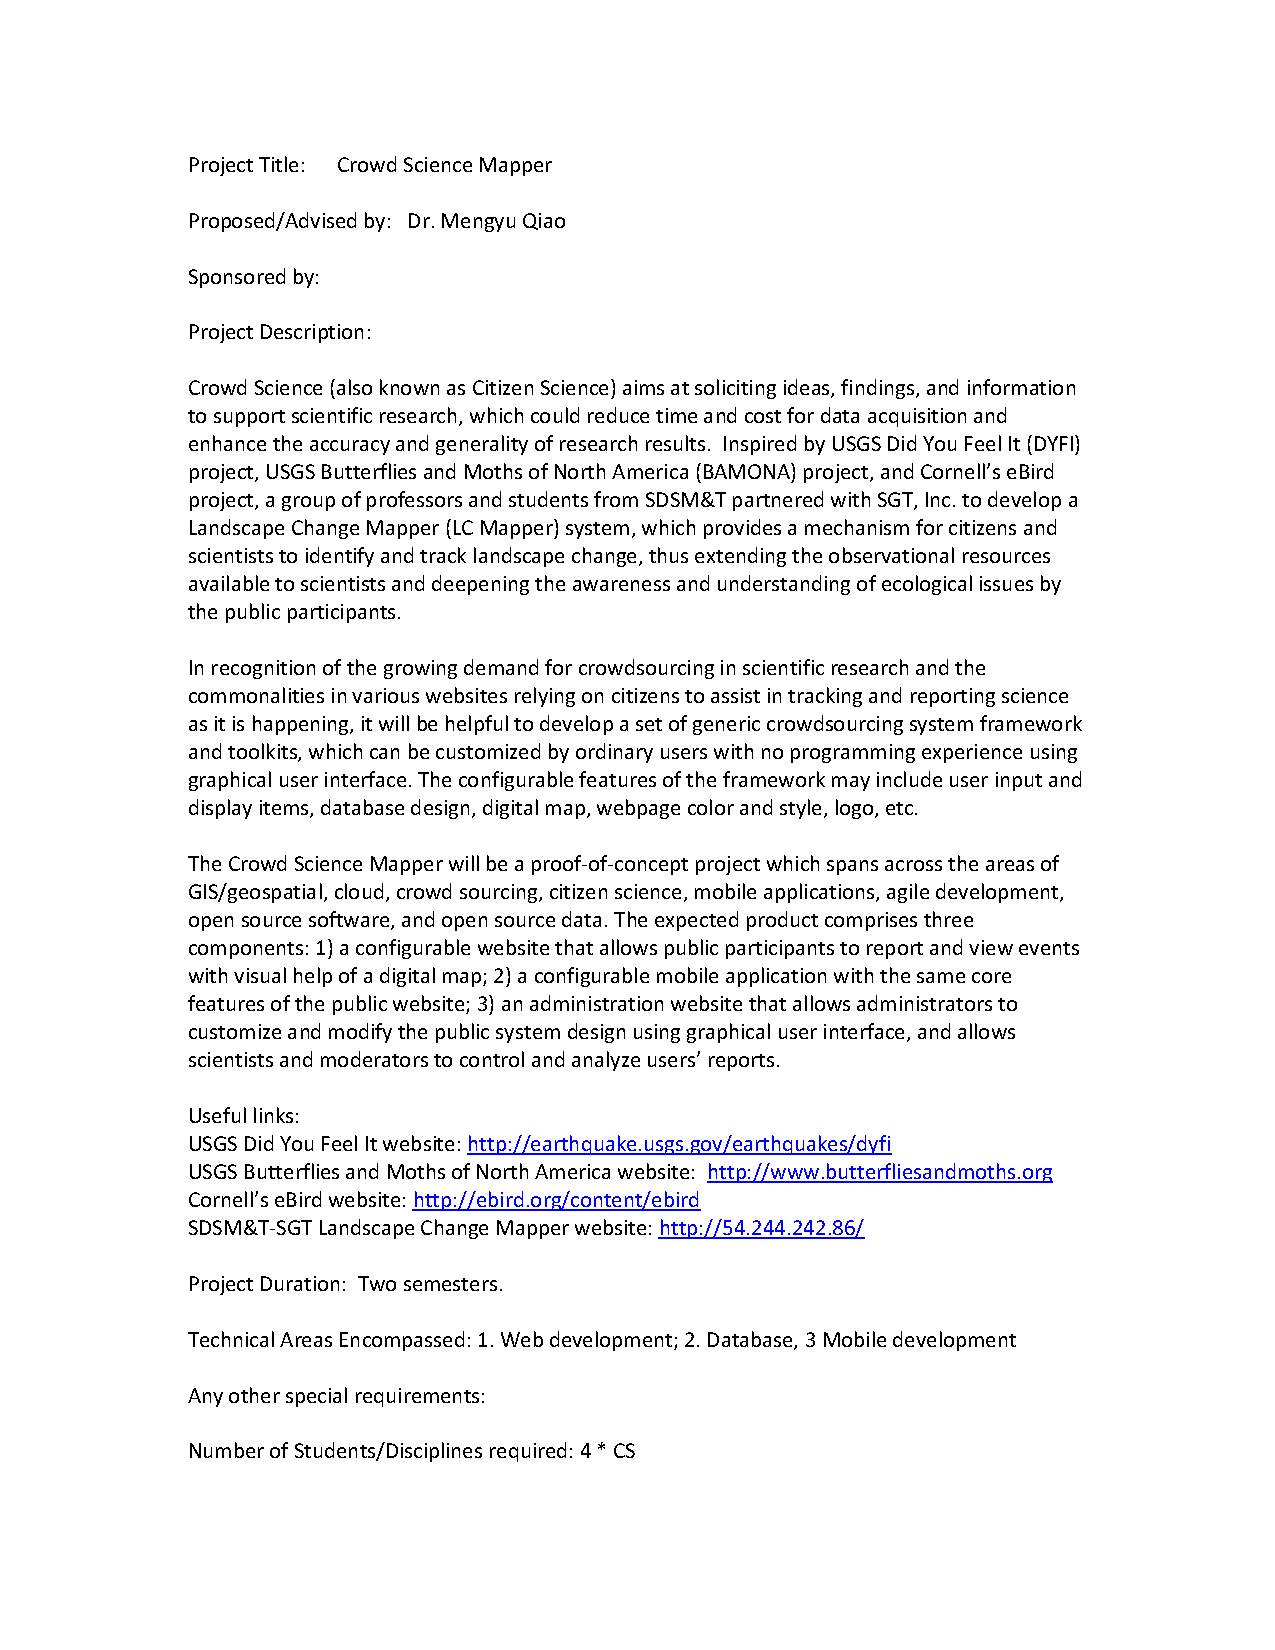
\includepdf[pages={1-1}]{CrowdScienceMapperProjectDescription.pdf}
\end{document}
